%%%%%%%%%%%%%%%%%%%%%%%%%%%%%%%%%%%%%%%%%%%%%%%%%%%%%%%%%%%%%%%%%%%%%%
% LaTeX Template: Beamer arrows
%
% Source: http://www.texample.net/
% Feel free to distribute this template, but please keep the
% referal to TeXample.net.
% Date: Nov 2006
% 
%%%%%%%%%%%%%%%%%%%%%%%%%%%%%%%%%%%%%%%%%%%%%%%%%%%%%%%%%%%%%%%%%%%%%%
% How to use writeLaTeX: 
%
% You edit the source code here on the left, and the preview on the
% right shows you the result within a few seconds.
%
% Bookmark this page and share the URL with your co-authors. They can
% edit at the same time!
%
% You can upload figures, bibliographies, custom classes and
% styles using the files menu.
%
% If you're new to LaTeX, the wikibook is a great place to start:
% http://en.wikibooks.org/wiki/LaTeX
%
%%%%%%%%%%%%%%%%%%%%%%%%%%%%%%%%%%%%%%%%%%%%%%%%%%%%%%%%%%%%%%%%%%%%%%

\documentclass{beamer} %
\usetheme{CambridgeUS}
\usepackage[utf8]{inputenc}
\usefonttheme{professionalfonts}
\usepackage{times}
\usepackage{tikz}
\usepackage{amsmath}
\usepackage{verbatim}
\usepackage{multicol}
\usetikzlibrary{arrows,shapes}
\usepackage{subfig}
\usepackage{booktabs}
\usepackage{cite}
\usepackage{graphicx}
\graphicspath{{../../Figures/presentation_19_05/}{../../Images/presentation_19_05/}}
\author{Danilo Fernandes}
\title{Processamento e análise de grandes imagens PolSAR}
\date{Maio, 2019}

\begin{document}

% For every picture that defines or uses external nodes, you'll have to
% apply the 'remember picture' style. To avoid some typing, we'll apply
% the style to all pictures.
\tikzstyle{every picture}+=[remember picture]

% By default all math in TikZ nodes are set in inline mode. Change this to
% displaystyle so that we don't get small fractions.
\everymath{\displaystyle}

\begin{frame}
    \titlepage
\end{frame}

\begin{frame}
\frametitle{Introdução}

Principais características das imagens PolSAR (\textit{Polarimetric Synthetic Aperture Radar}):
\begin{itemize}
    \item Uso de ondas eletromagnéticas no espectro das microondas;% -- com frequência e comprimento de onda que variam de 0.3 GHz e 100 cm a 100GHz e 0.3cm;
    \item Descrevem a estrutura geométrica e propriedades dielétricas dos objetos imageados na relação entre a polarização das ondas incidentes e refletidas.
\end{itemize}

\end{frame}

\begin{frame}
\frametitle{Introdução}

Vantagens em relação a sistemas de imageamento ótico:

\begin{itemize}
    \item Independência de iluminação solar;
    \item Independência de fatores climáticos.
\end{itemize}

\end{frame}

\begin{frame}
\frametitle{Introdução}

Equações de Maxwell:

\vspace{0.05\linewidth}

\noindent
\begin{minipage}{.5\linewidth}
\begin{equation}
  \boldsymbol{\nabla} \cdot \mathbf{E} = \frac{\rho}{\varepsilon_0}
\end{equation}
\end{minipage}%
\begin{minipage}{.5\linewidth}
\begin{equation}
 \boldsymbol{\nabla} \cdot \mathbf{B} = 0
\end{equation}
\end{minipage}

\vspace{0.05\linewidth}

\noindent
\begin{minipage}{.5\linewidth}
\begin{equation}
  \boldsymbol{\nabla} \times \mathbf{E} =  -\frac{\partial \mathbf{B}}{\partial t}
\end{equation}
\end{minipage}%
\begin{minipage}{.5\linewidth}
\begin{equation}
 \boldsymbol{\nabla} \times \mathbf{B} = \mu_0 \mathbf{J} + \varepsilon_0 \mu_0 \frac{\partial \mathbf{E}}{\partial t}
\end{equation}
\end{minipage}

\vspace{0.05\linewidth}
Equação de onda:

\vspace{0.05\linewidth}
\noindent
\begin{minipage}{.5\linewidth}
    \begin{equation}
        \nabla^2 \mathbf{E} - \mu_0 \varepsilon_0 \frac{\partial^2 \mathbf{E}}{\partial t^2} = 0
    \end{equation}
\end{minipage}%
\noindent
\begin{minipage}{.5\linewidth}
    \begin{equation}
        \nabla^2 \mathbf{B} - \mu_0 \varepsilon_0 \frac{\partial^2 \mathbf{B}}{\partial t^2} = 0
    \end{equation}
\end{minipage}
\end{frame}

\begin{frame}{Introdução}
    Solução para as equações 5:
    
    \begin{displaymath}
       \mathbf{E} =
        \begin{bmatrix}
             E_x \cos(\omega t - kz + \delta_x)\\
             E_y \cos(\omega t - kz + \delta_y)
        \end{bmatrix}
        = \Re
        \begin{Bmatrix}
            \begin{bmatrix}
                 E_x e^{j(\omega t - kz + \delta_x)}\\
                 E_y e^{j(\omega t - kz + \delta_y)}
            \end{bmatrix}
        \end{Bmatrix}
    \end{displaymath}
    
    \begin{displaymath}
        = \Re
            \begin{Bmatrix}
                \begin{bmatrix}
                     E_x e^{j\delta_x}\\
                     E_y e^{j\delta_y}
                \end{bmatrix}
                e^{j(\omega t - kz)}
            \end{Bmatrix}
    \end{displaymath}
    
    \vspace{0.05\linewidth}
    
    onde $e^{j\alpha} = \cos \alpha + j\sin \alpha$ e $E =$ 
    $
    \begin{bmatrix}
         E_x e^{j\delta_x}\\
         E_y e^{j\delta_y}
    \end{bmatrix}
    $
    é chamado Vetor de Jones~\cite{Pottier09}.

\end{frame}

\begin{frame}{Introdução}
   
   \begin{figure}
           \centering
           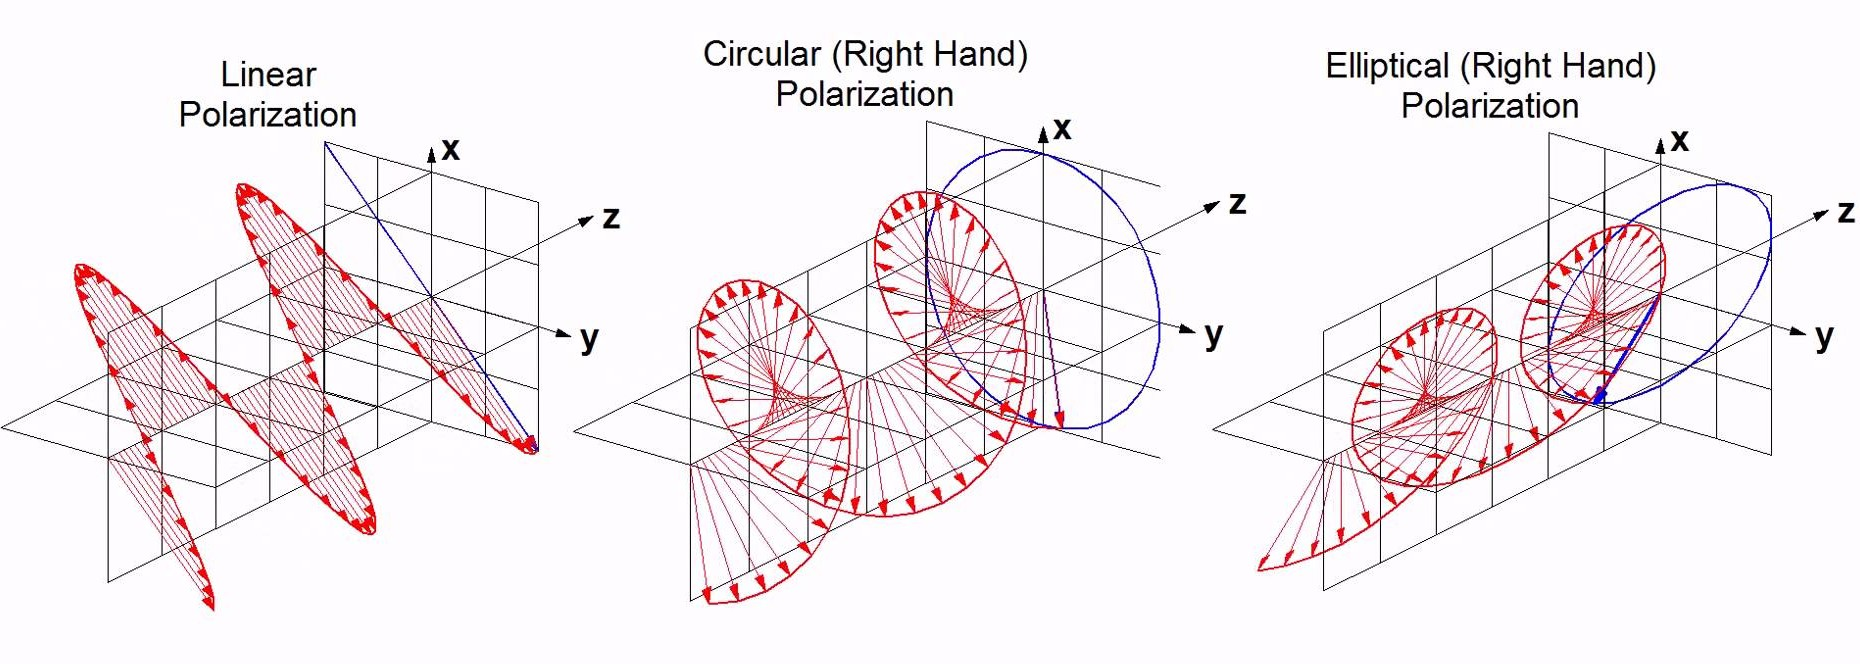
\includegraphics[width = .9\linewidth]{eletro_wave.jpg}
           \caption{Da esquerda para a direita temos: $E_y = E_x$ e $\delta_x = \delta_y$; $E_y = E_x$ e $\delta_x = \delta_y + \pi/2$; $E_y \neq E_x$ e $\delta_x = \delta_y + \pi/2$ }
           \label{fig:eletro_wave}
    \end{figure}
    
\end{frame}

\begin{frame}{Introdução}
    Temos que um pixel de uma imagem PolSAR \textit{Single Look} consiste na matriz de retroespalhamento $S$ tal que~\cite{Pottier09}:
    
    \begin{equation}
        E_S = S E_I
    \end{equation}
    
    \begin{equation}
        S = 
        \begin{bmatrix}
            S_{HH} & S_{HV}\\
            S_{VH} & S_{VV}
        \end{bmatrix}
    \end{equation}
    
    onde $E_S$ e $E_I$ correspondem às ondas refletida e incidente, respectivamente.
\end{frame}

\begin{frame}{Introdução}
    Um pixel de uma imagem PolSAR \textit{Multilook} consiste na matriz de covariância $C$ tal que~\cite{Pottier09}:
    
    \begin{equation}
        T = \frac{1}{L} \sum_{i=1}^L k^H_i k_i 
    \end{equation}
    
    para $k$ = [$S_{HH}$ $S_{HV}$  $S_{VV}$].
\end{frame}

\begin{frame}{Introdução}
    
    \begin{figure}%
        \centering
        \subfloat[\textit{Single Look}]{{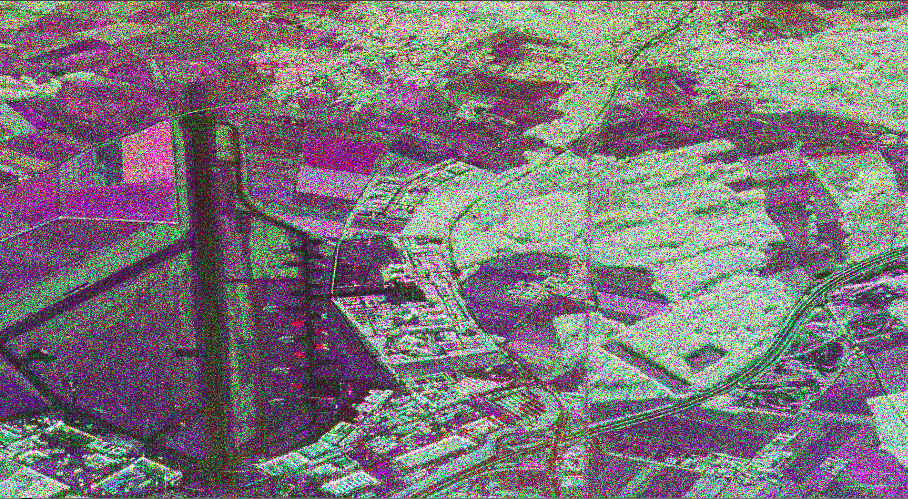
\includegraphics[width = .45\linewidth]{oberpfaffenhofen_trad_algorithm_reduced.png} }}%
        \qquad
        \subfloat[\textit{Multilook}]{{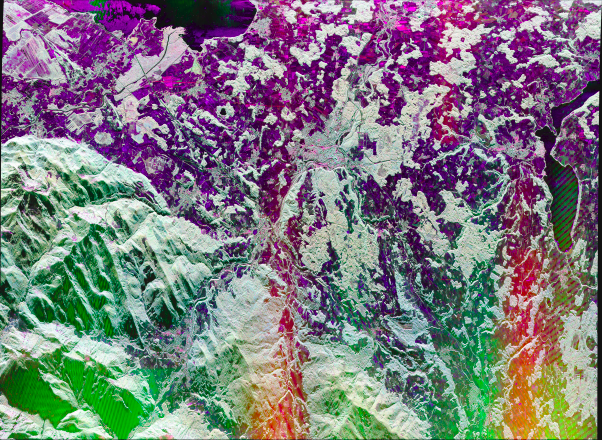
\includegraphics[width=.45\linewidth]{traunstein_trad_algorithm_reduced.png} }}%
        \caption{Visualização de imagens PolSAR através dos dados de intensidade}%
        \label{fig:example}%
    \end{figure}
    
\end{frame}

\begin{frame}{Distância Geodésica}

Dada a matriz de covariância $T$, a sua correspondente matriz de Kennaugh $K$ é dada por~\cite{ClassificationPolSARGeodesic}:


\scriptsize
\begin{equation}
K =
\begin{bmatrix}
\frac{ T_{11} + T_{22} + T_{33} }{2} & \Re(T_{12}) & \Re(T_{13}) & \Im(T_{23})\\
\Re(T_{12}) & \frac{T_{11} + T_{22} - T_{33}}{2} & \Re(T_{23}) & \Im(T_{13})\\
\Re(T_{13}) & \Re(T_{23}) & \frac{ T_{11} - T_{22} + T_{33} }{2} & -\Im(T_{12})\\
\Im(T_{23}) & \Im(T_{13}) & -\Im(T_{12}) & \frac{ -T_{11} + T_{22} + T_{33} }{2}\\
\end{bmatrix}
\end{equation}

\normalsize
    
\end{frame}

\begin{frame}{Distância Geodésica}
    Dada as matrizes de Kennaugh $K_1$ e $K_2$, é possível medir a distância entre as mesmas -- usando a Distância Geodésica -- da seguinte forma~\cite{ClassificationPolSARGeodesic}:
    
    \begin{equation}
GD(K_1, K_2) = \frac{2}{\pi} \cos^{-1} \left(\frac{Tr(K_1^T K_2)}{\sqrt{Tr(K_1^T K_1)} \sqrt{Tr(K_2^T K_2})} \right).
\end{equation}

onde $GD(K_1, K_2) \in [0,1]$.
    
\end{frame}

\begin{frame}{Histogramas das similaridades em relação aos retroespalhadores elementares}

\begin{figure}
    \centering
    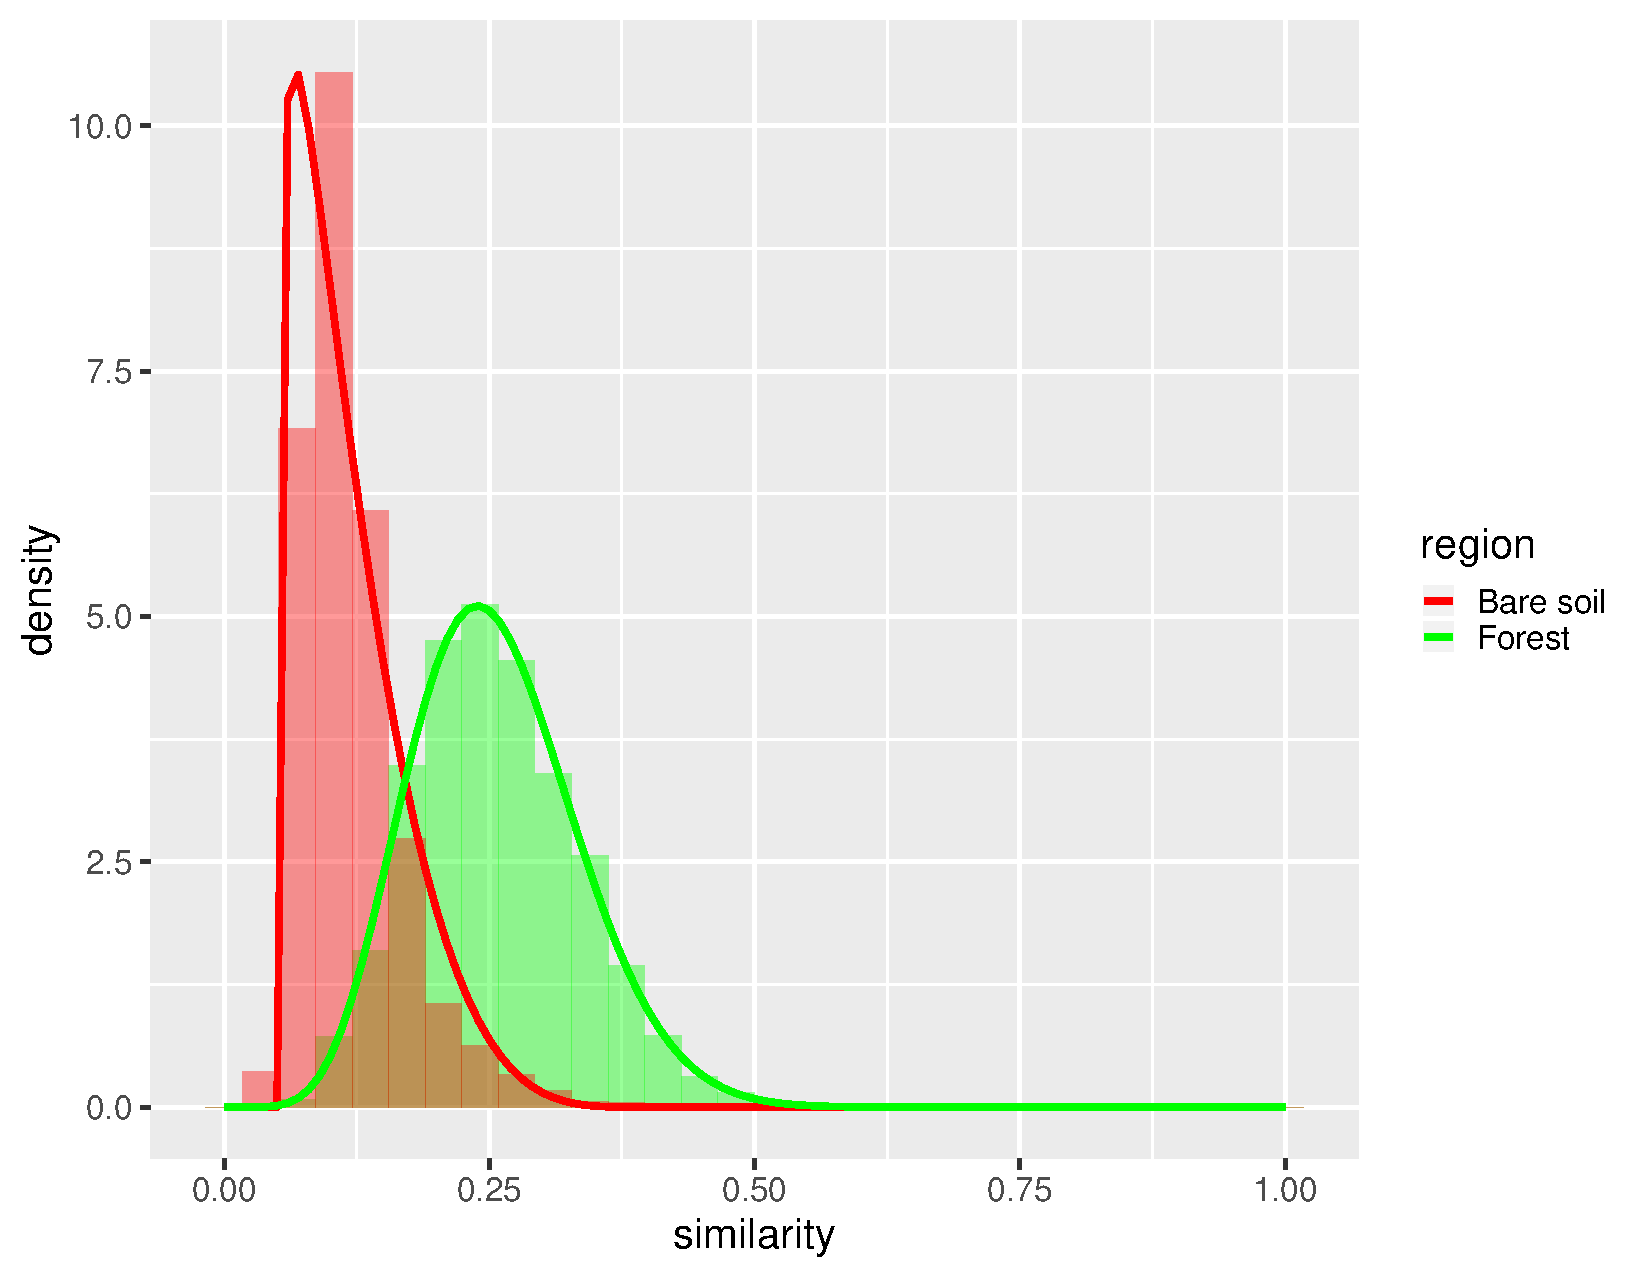
\includegraphics[width = .6\linewidth]{wvn.pdf}
    \caption{Simaridade entre os dados PolSAR de regiões de vegetação e solo exposta em relação ao retroespalhador elementar \textit{-1/4-wave}}
    \label{fig:wvn}
\end{figure}
    
\end{frame}

\begin{frame}{Histogramas das similaridades em relação aos retroespalhadores elementares}

\begin{figure}
    \centering
    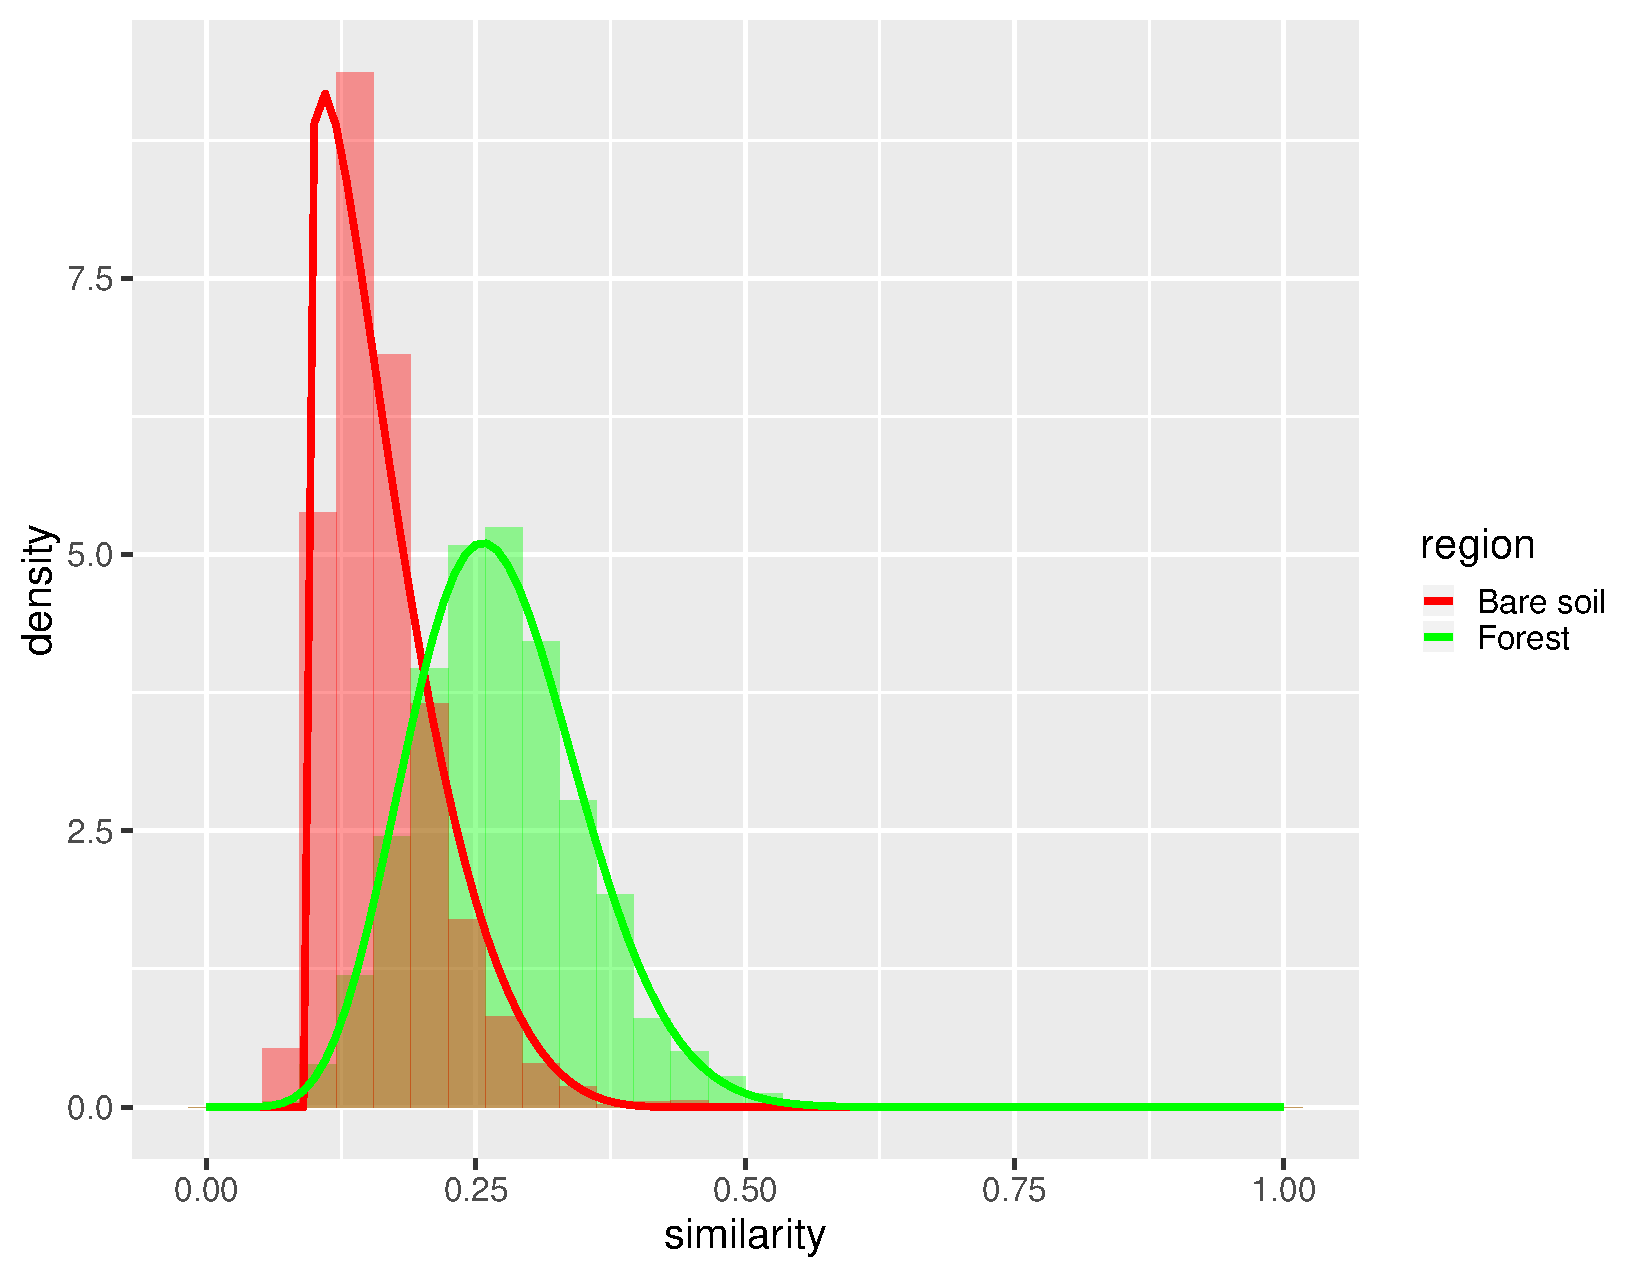
\includegraphics[width = .6\linewidth]{wvp.pdf}
    \caption{Simaridade entre os dados PolSAR de regiões de vegetação e solo exposta em relação ao retroespalhador elementar \textit{+1/4-wave}}
    \label{fig:wvp}
\end{figure}
    
\end{frame}

\begin{frame}{Histogramas das similaridades em relação aos retroespalhadores elementares}

\begin{figure}
    \centering
    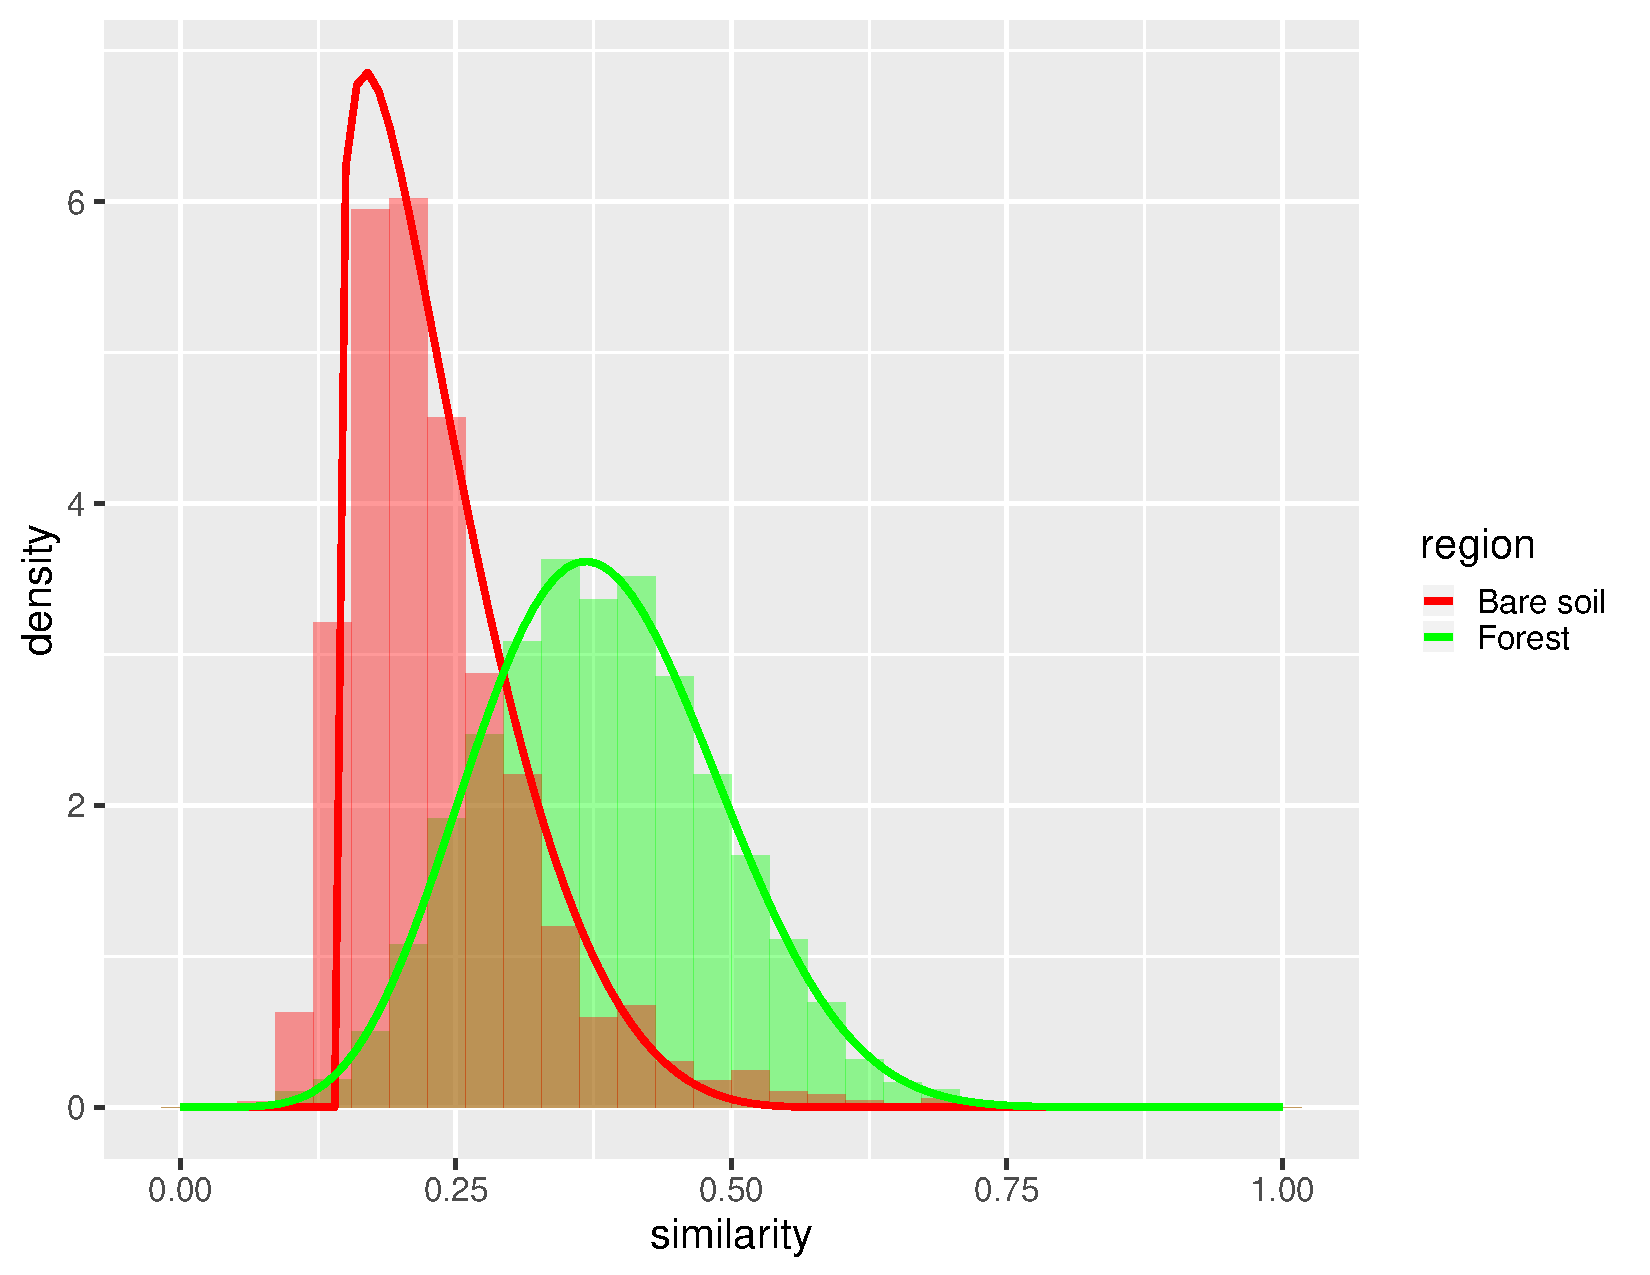
\includegraphics[width = .6\linewidth]{cy.pdf}
    \caption{Simaridade entre os dados PolSAR de regiões de vegetação e solo exposta em relação ao retroespalhador elementar \textit{cylinder}}
    \label{fig:cy}
\end{figure}
    
\end{frame}

\begin{frame}{Histogramas das similaridades em relação aos retroespalhadores elementares}

\begin{figure}
    \centering
    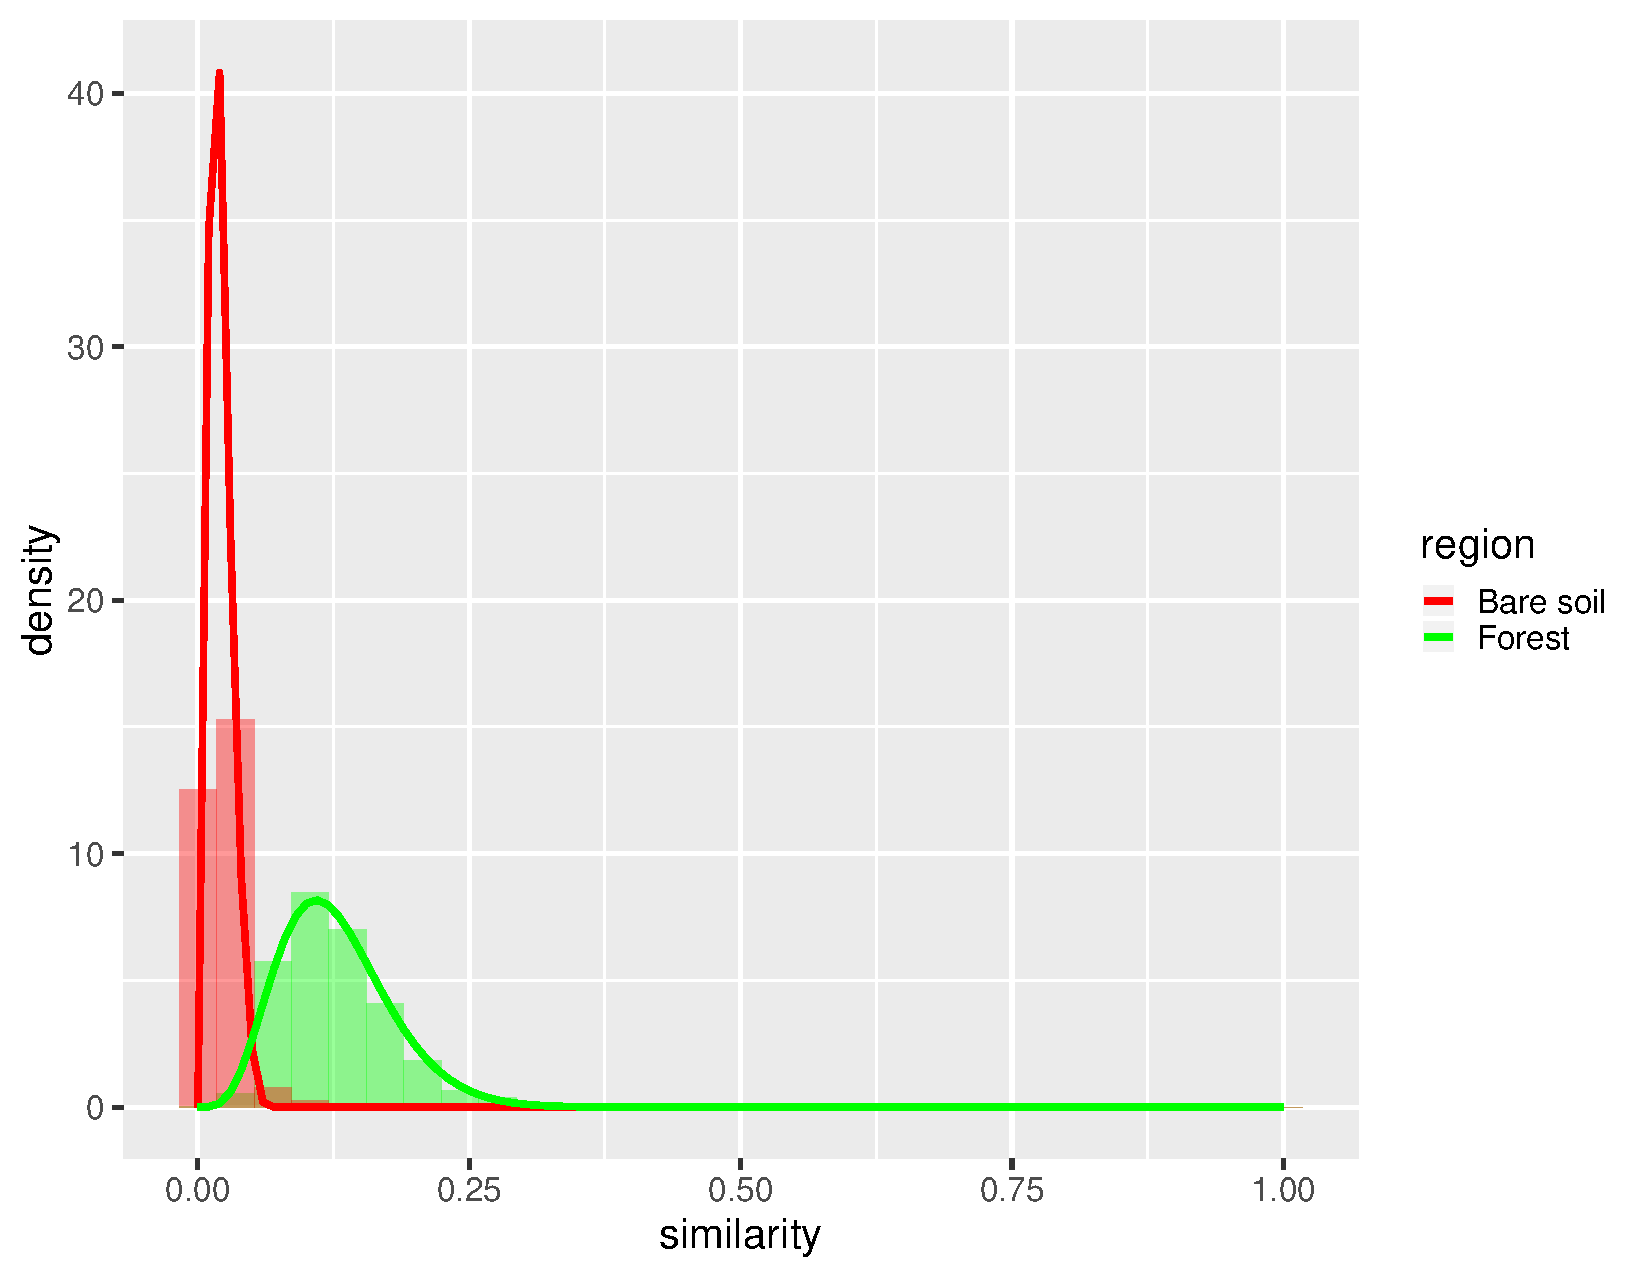
\includegraphics[width = .6\linewidth]{di.pdf}
    \caption{Simaridade entre os dados PolSAR de regiões de vegetação e solo exposta em relação ao retroespalhador elementar \textit{dihedral}}
    \label{fig:di}
\end{figure}
    
\end{frame}

\begin{frame}{Histogramas das similaridades em relação aos retroespalhadores elementares}

\begin{figure}
    \centering
    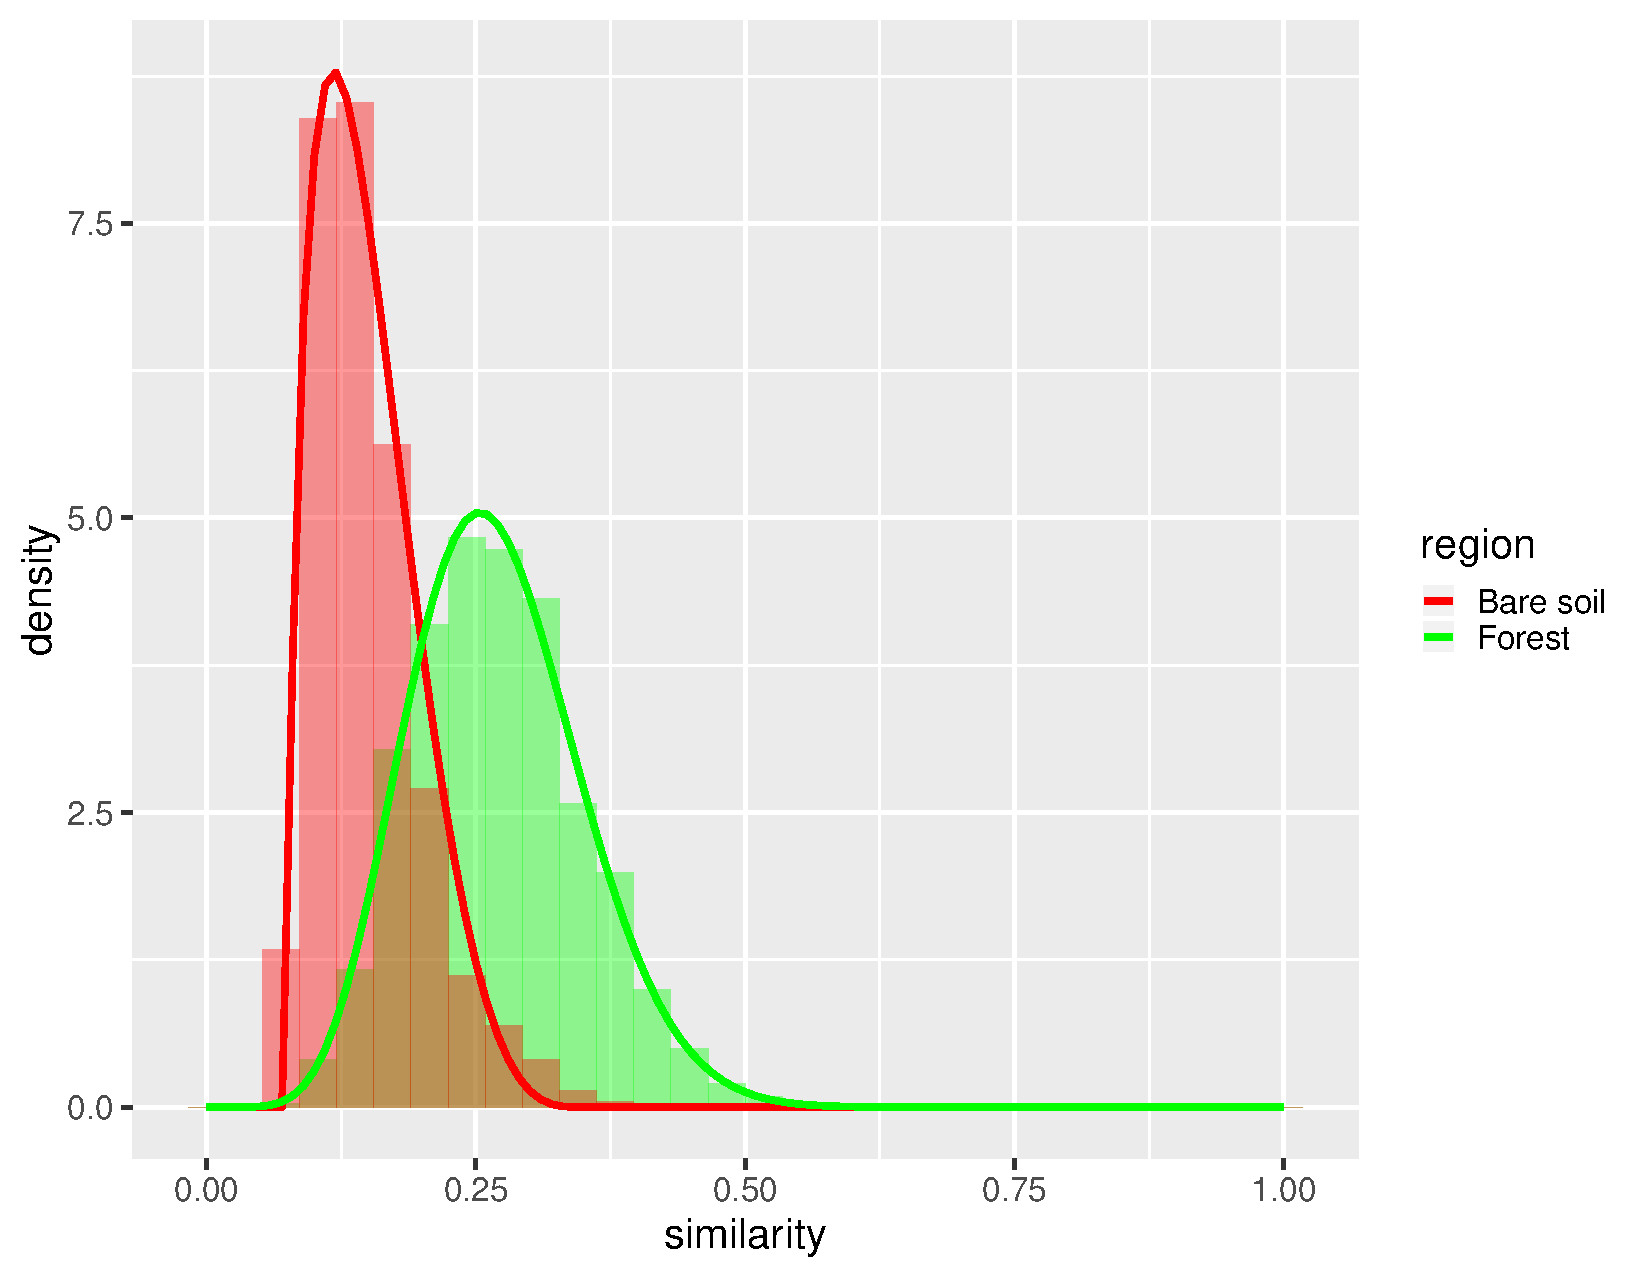
\includegraphics[width = .6\linewidth]{dip.pdf}
    \caption{Simaridade entre os dados PolSAR de regiões de vegetação e solo exposta em relação ao retroespalhador elementar \textit{dipole}}
    \label{fig:dip}
\end{figure}
    
\end{frame}

\begin{frame}{Histogramas das similaridades em relação aos retroespalhadores elementares}

\begin{figure}
    \centering
    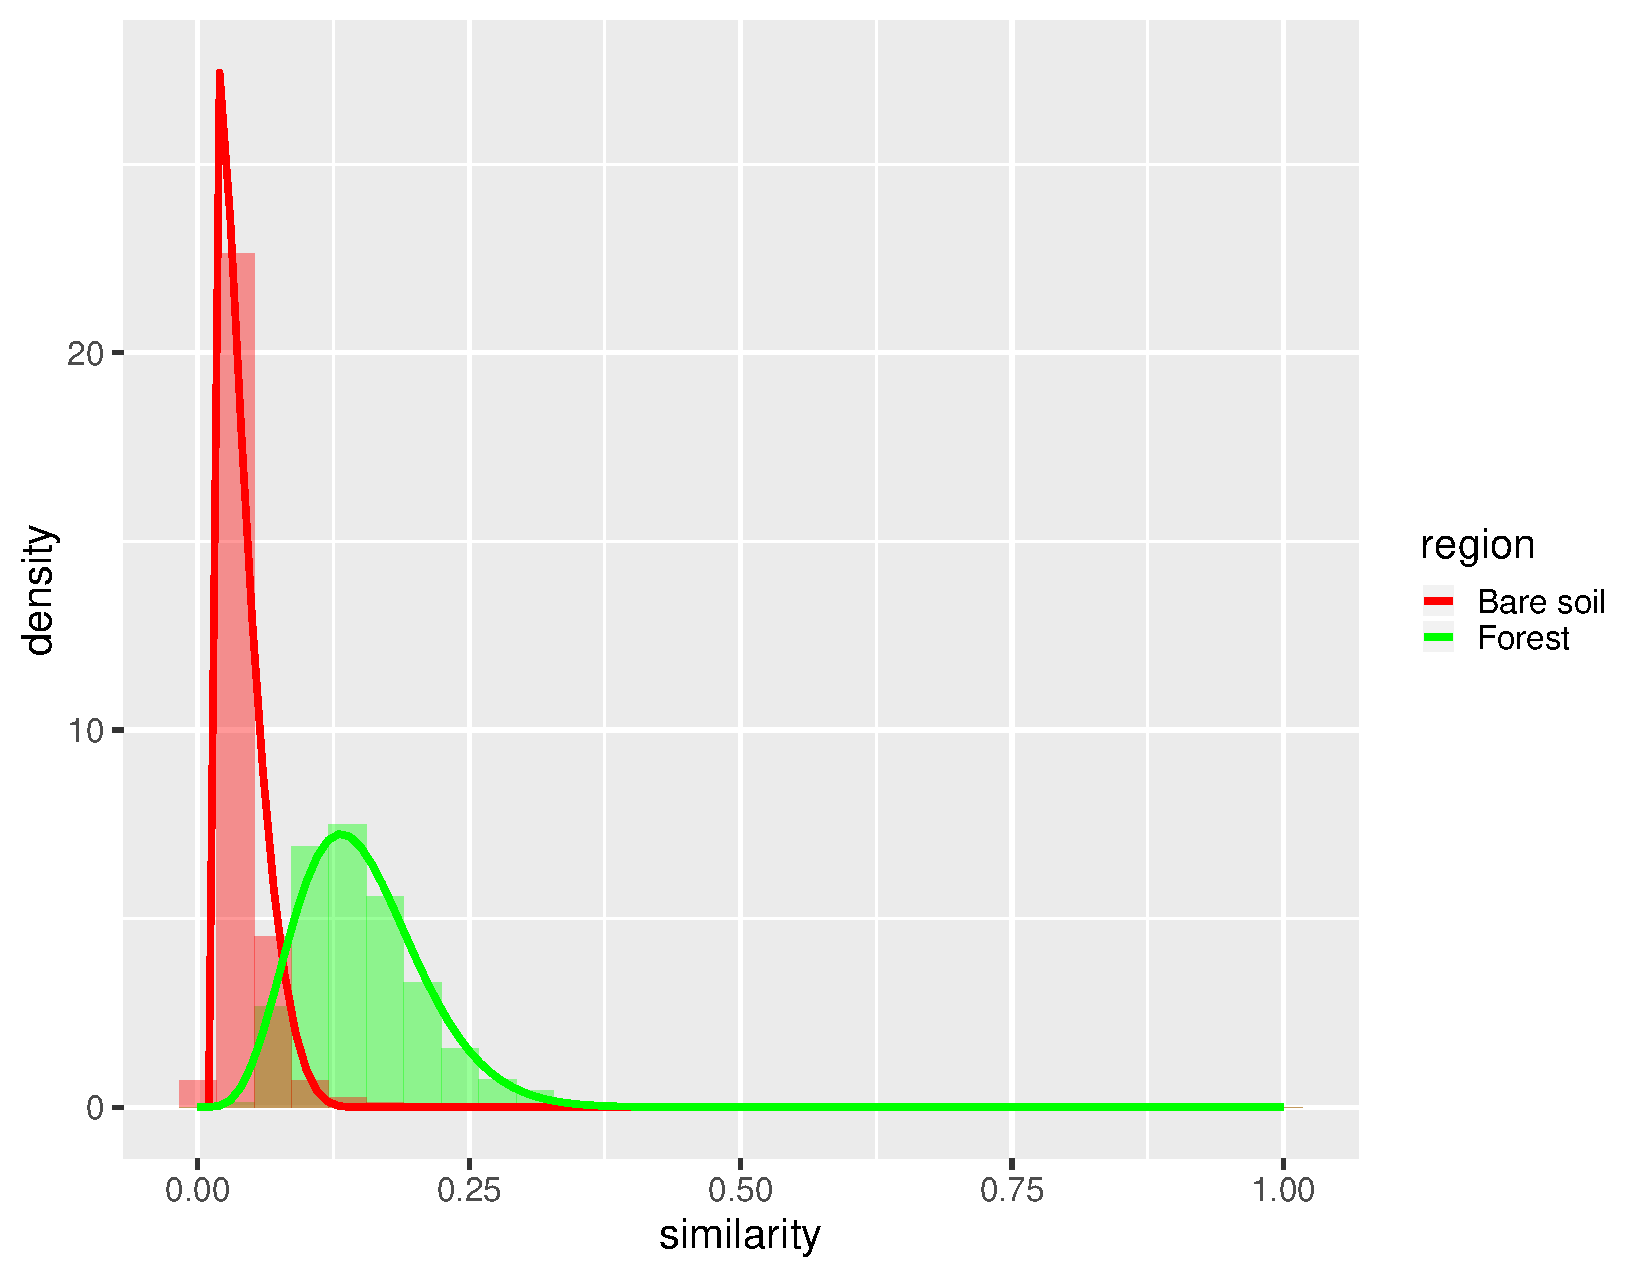
\includegraphics[width = .6\linewidth]{nd.pdf}
    \caption{Simaridade entre os dados PolSAR de regiões de vegetação e solo exposta em relação ao retroespalhador elementar \textit{narrow dihedral}}
    \label{fig:nd}
\end{figure}
    
\end{frame}

\begin{frame}{Histogramas das similaridades em relação aos retroespalhadores elementares}

\begin{figure}
    \centering
    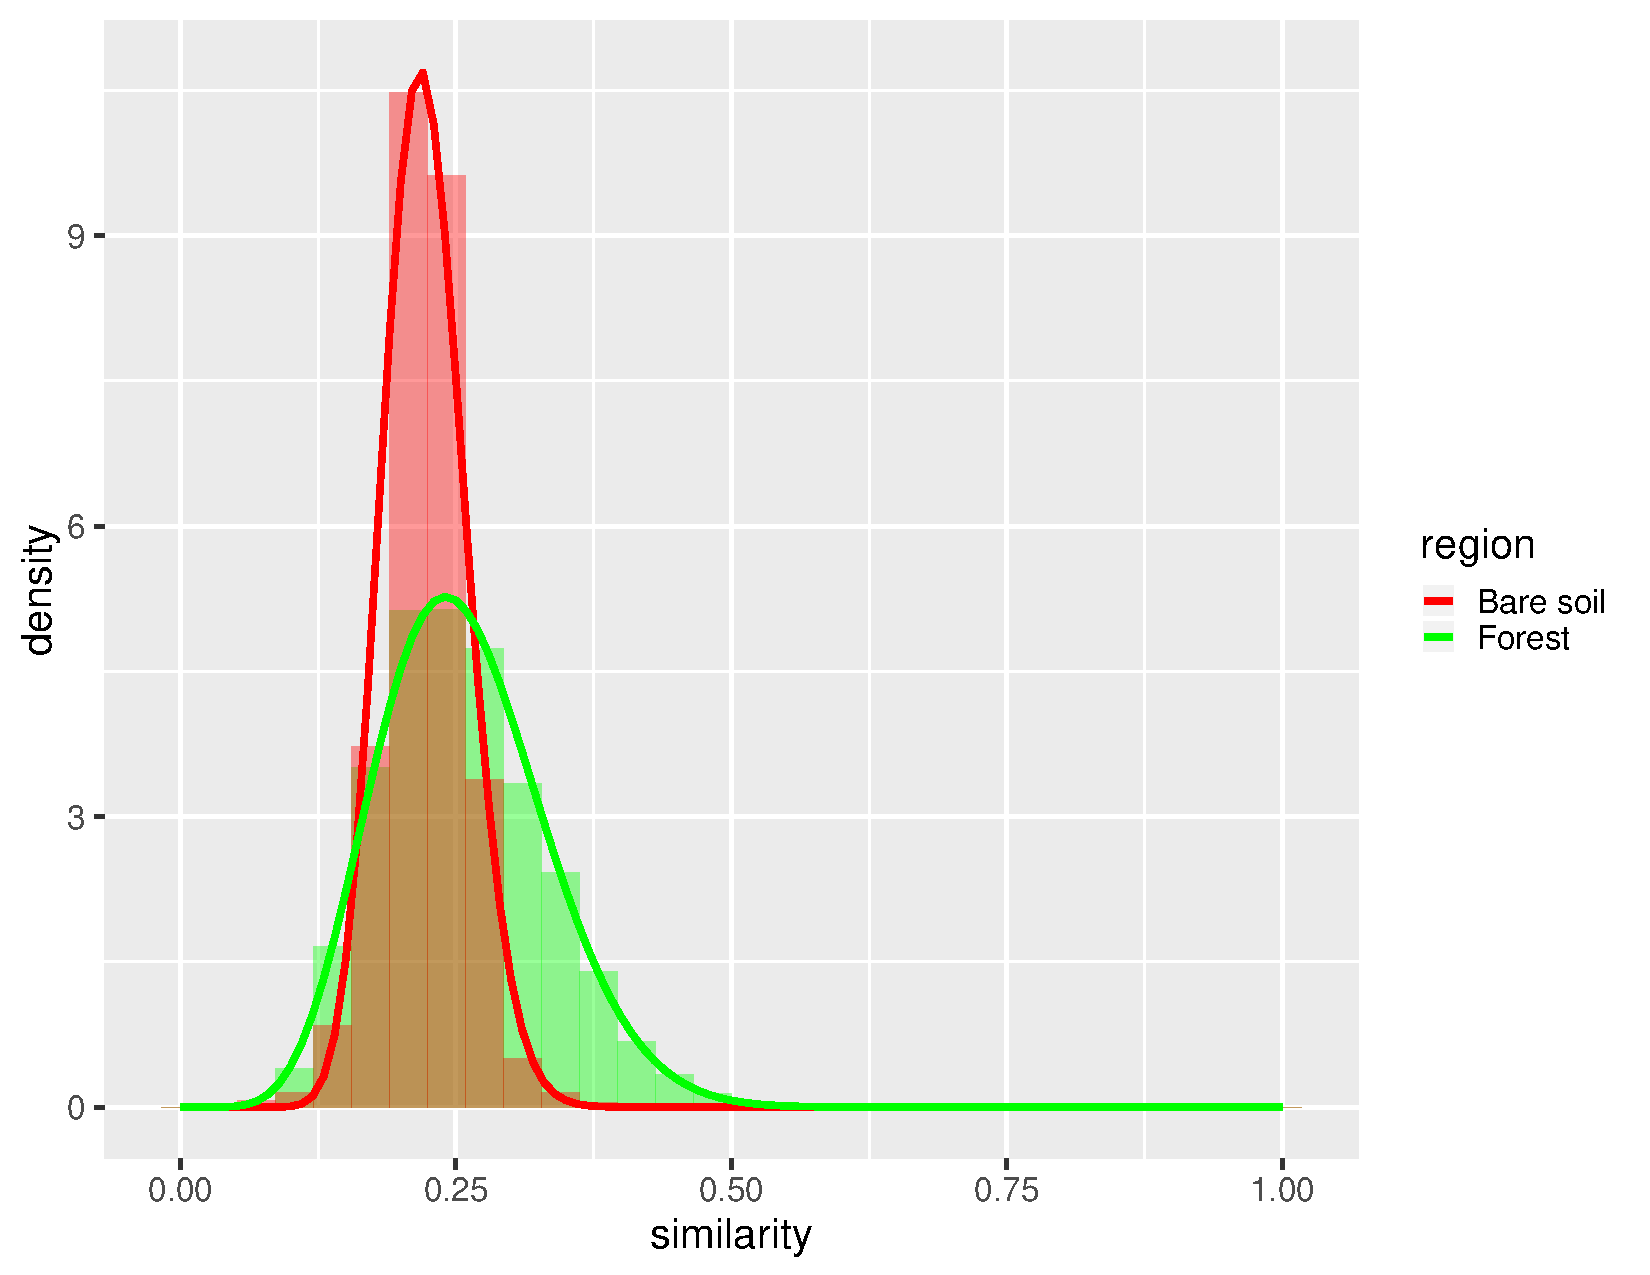
\includegraphics[width = .6\linewidth]{lh.pdf}
    \caption{Simaridade entre os dados PolSAR de regiões de vegetação e solo exposta em relação ao retroespalhador elementar \textit{left helix}}
    \label{fig:lh}
\end{figure}
    
\end{frame}

\begin{frame}{Histogramas das similaridades em relação aos retroespalhadores elementares}

\begin{figure}
    \centering
    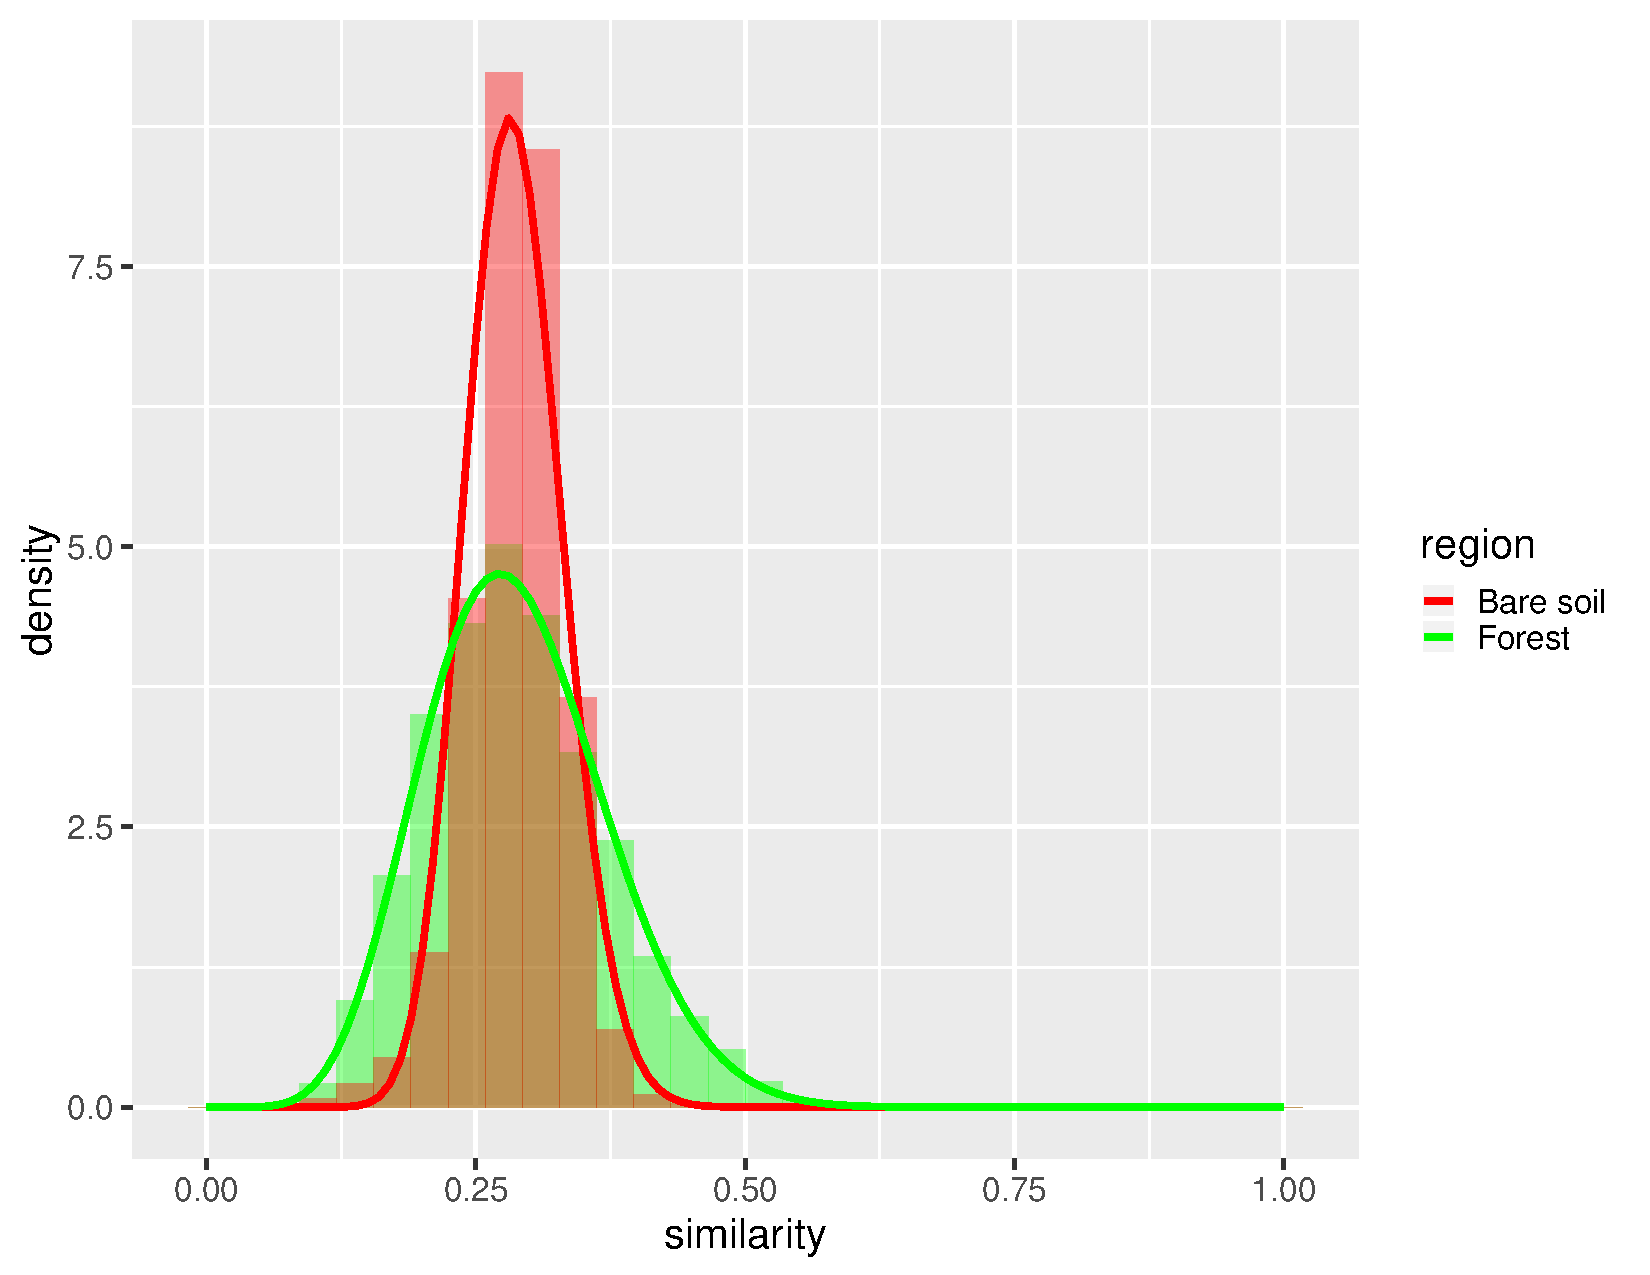
\includegraphics[width = .6\linewidth]{rh.pdf}
    \caption{Simaridade entre os dados PolSAR de regiões de vegetação e solo exposta em relação ao retroespalhador elementar \textit{right helix}}
    \label{fig:rh}
\end{figure}
    
\end{frame}

\begin{frame}{Histogramas das similaridades em relação aos retroespalhadores elementares}

\begin{figure}
    \centering
    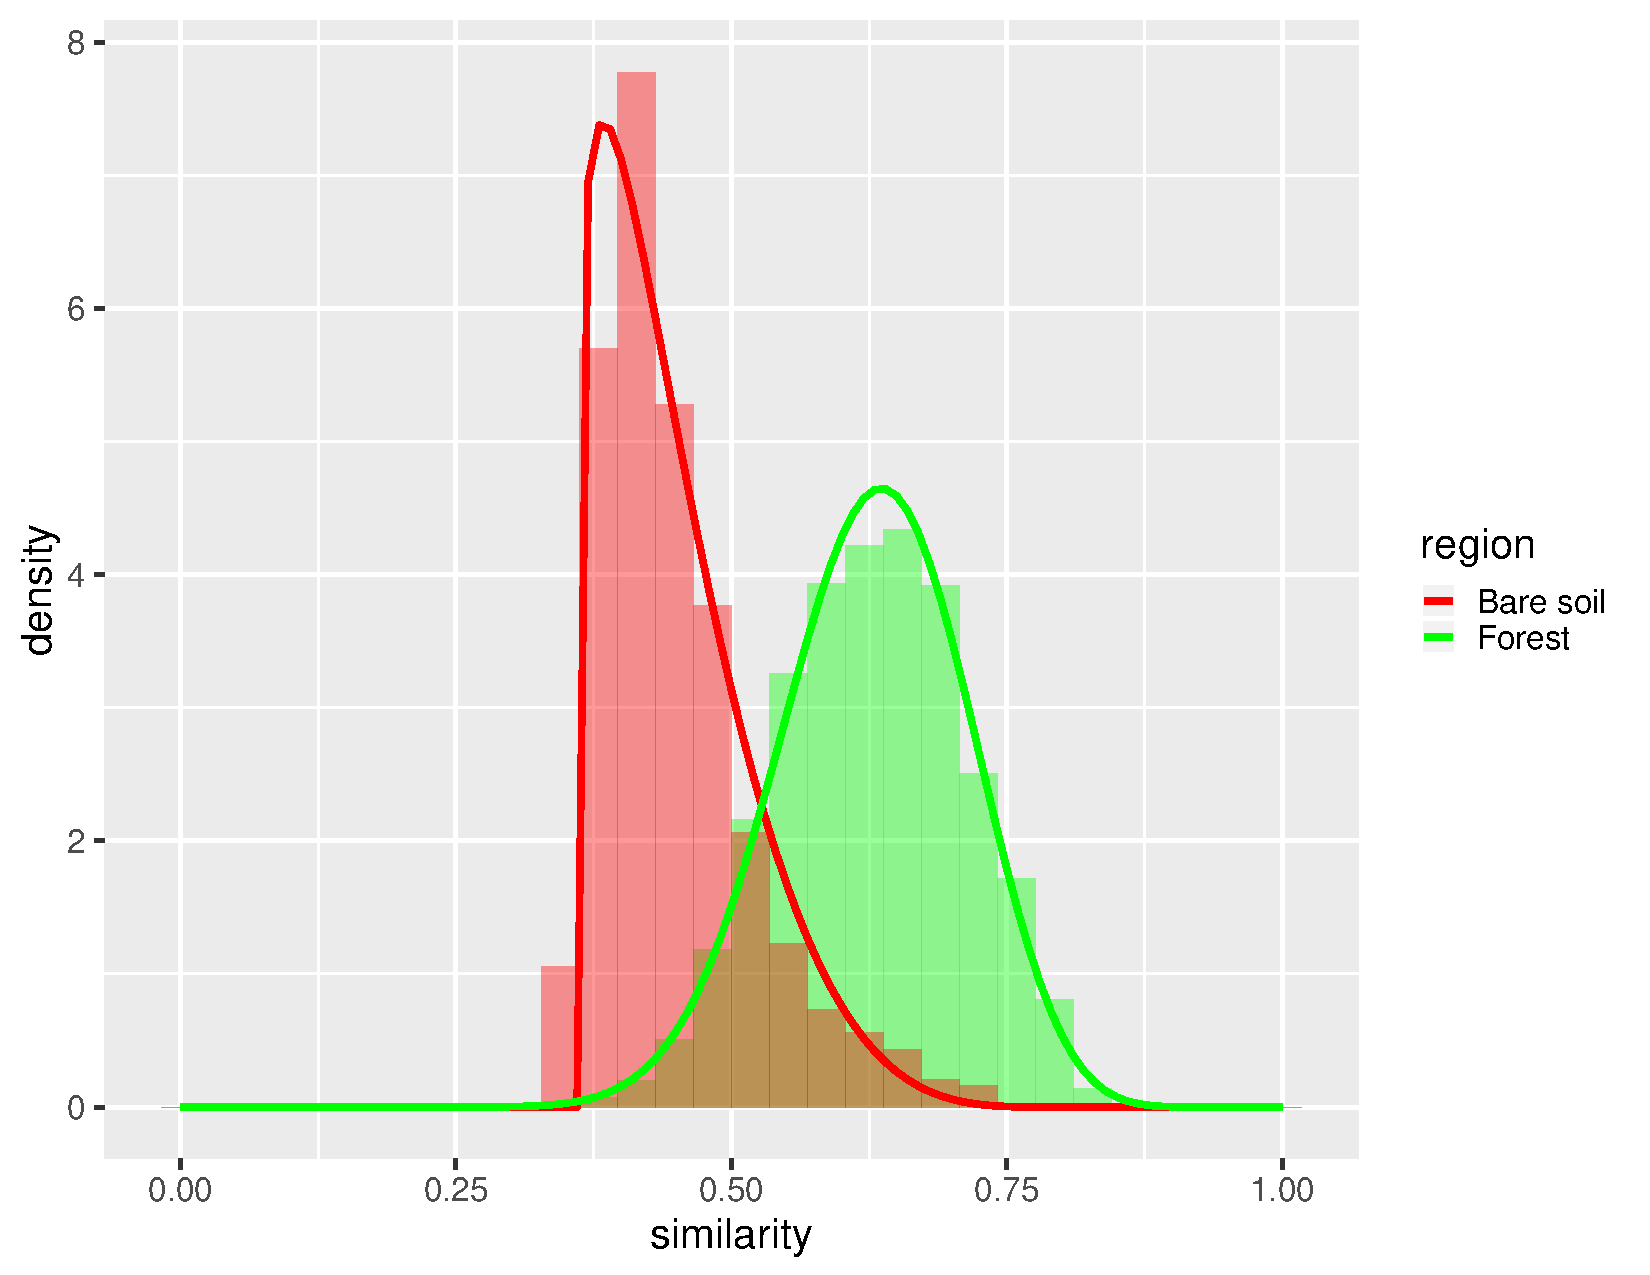
\includegraphics[width = .6\linewidth]{rv.pdf}
    \caption{Simaridade entre os dados PolSAR de regiões de vegetação e solo exposta em relação ao retroespalhador elementar \textit{random volume}}
    \label{fig:rv}
\end{figure}
    
\end{frame}

\begin{frame}{Histogramas das similaridades em relação aos retroespalhadores elementares}

\begin{figure}
    \centering
    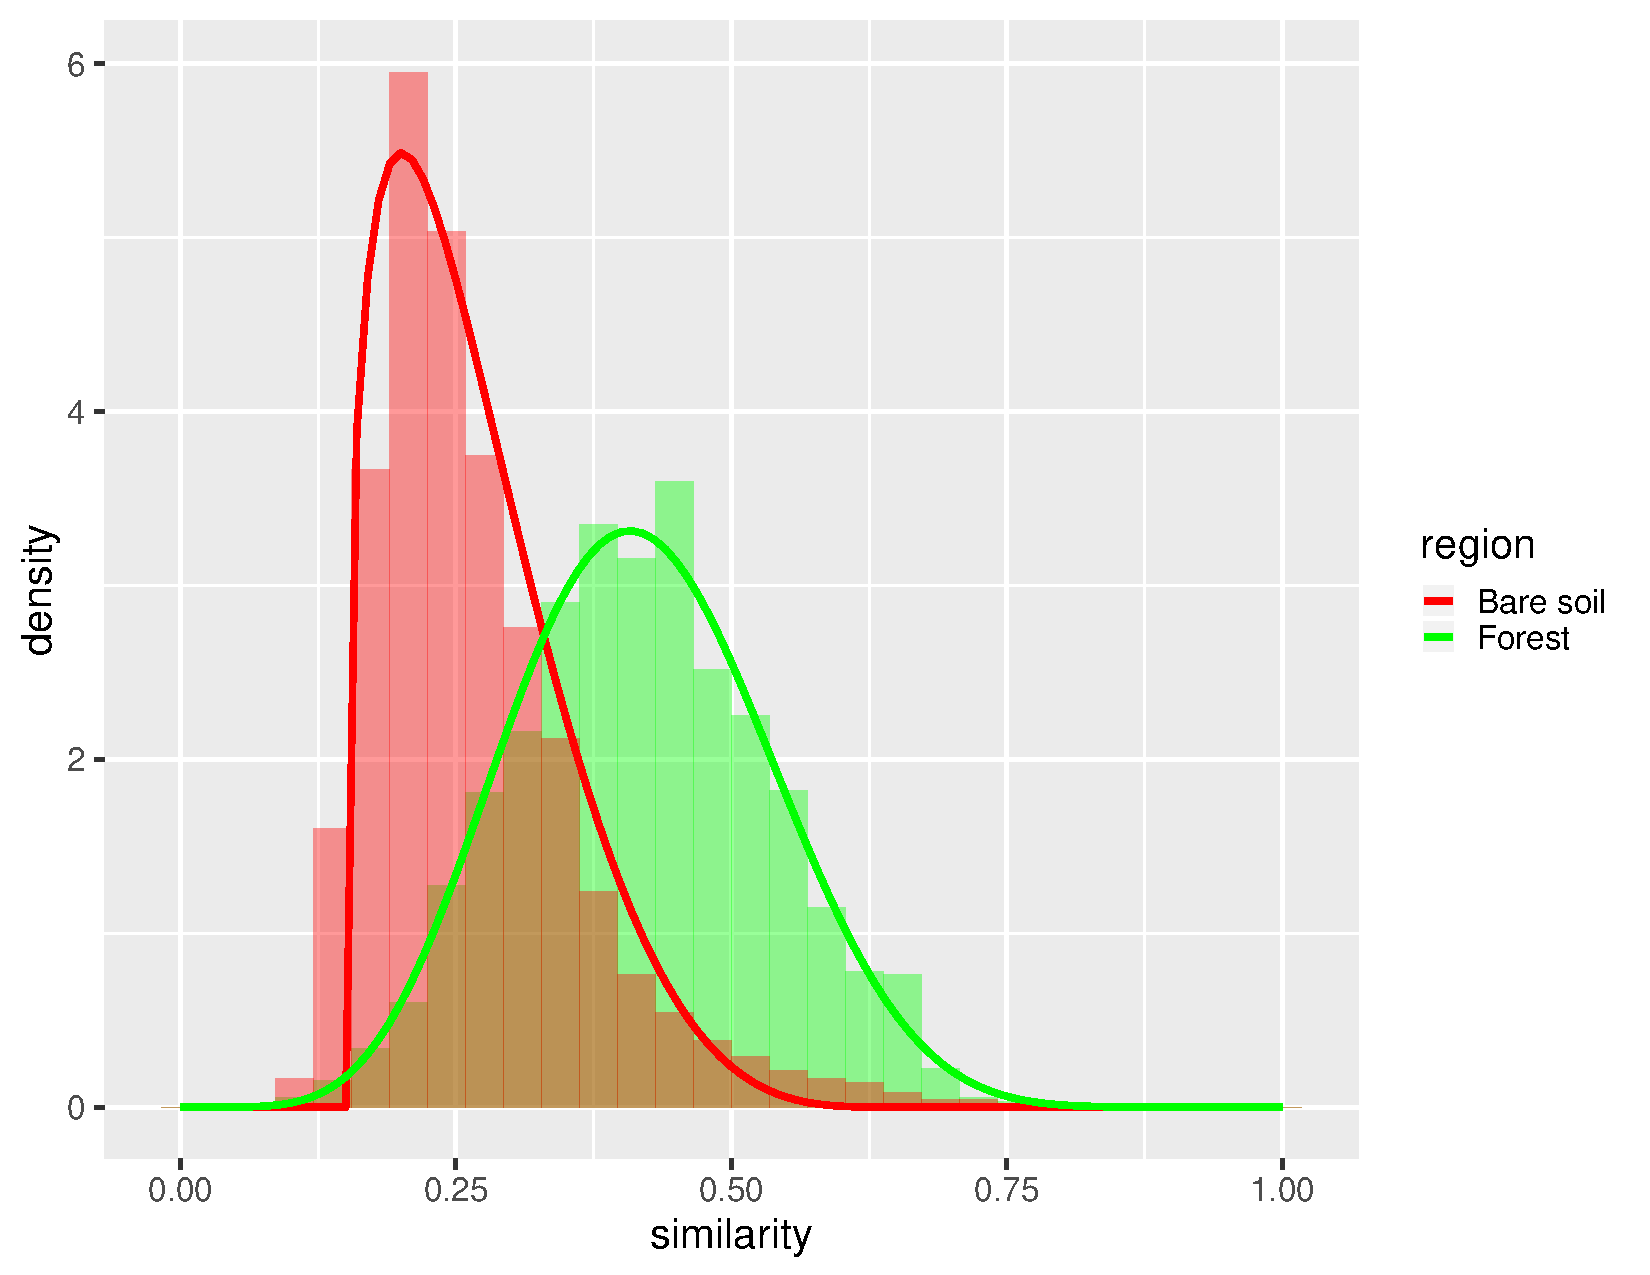
\includegraphics[width = .6\linewidth]{tr.pdf}
    \caption{Simaridade entre os dados PolSAR de regiões de vegetação e solo exposta em relação ao retroespalhador elementar \textit{trihedral}}
    \label{fig:tr}
\end{figure}
    
\end{frame}

\begin{frame}{Distribuição Beta}

A função de densidade de probabilidade da distribuição beta é dada por:
$$
f(x) = \frac{\Gamma(\alpha+\beta)}{\Gamma(\alpha)\Gamma(\beta)(max - min)^{\alpha + \beta - 1}}(x - min)^{\alpha-1}(max-x)^{\beta-1},
$$
com $x \in [min, max]$, $\alpha,\beta>0$.
    
\end{frame}

\begin{frame}{Estimativa dos parâmetros da distribuição Beta e média para as similaridades analisadas}
\begin{table}[hbt]
\centering
%\caption{}\label{tab:estimated_params}     
\begin{tabular}{lrrrrr}
\toprule
& $\min$ & $\max$ & $\widehat\alpha$ & $\widehat\beta$ & $\widehat\mu$\\ \midrule
& \multicolumn{5}{c}{$-1/4$-wave}\\
\cmidrule(lr){2-6}
\textbf{Forest} & 0.000 & 1.000 & 7.830 & 22.758 & 0.255\\
\textbf{Bare soil} & 0.055 & 0.400 & 1.127 & 4.872 & 0.119\\
\midrule
%
& \multicolumn{5}{c}{$+1/4$-wave}\\
\cmidrule(lr){2-6}
\textbf{Forest} & 0.000 & 1.000 & 8.681 & 23.277 & 0.271\\
\textbf{Bare soil} & 0.090 & 0.450 & 1.200 & 4.800 & 0.162\\
\midrule
%
& \multicolumn{5}{c}{Cylinder}\\
\cmidrule(lr){2-6}
\textbf{Forest} & 0.000 & 1.000 & 7.500 & 12.165 & 0.381\\
\textbf{Bare soil} & 0.140 & 0.600 & 1.243 & 4.756 & 0.235\\
\bottomrule
\end{tabular}
\end{table}
\end{frame}

\begin{frame}{Estimativa dos parâmetros da distribuição Beta e média para as similaridades analisadas}
\begin{table}[hbt]
\centering
%\caption{}\label{tab:estimated_params}     
\begin{tabular}{lrrrrr}
\toprule
& $\min$ & $\max$ & $\widehat\alpha$ & $\widehat\beta$ & $\widehat\mu$\\ \midrule
& \multicolumn{5}{c}{Dihedral}\\
\cmidrule(lr){2-6}
\textbf{Forest} & 0.000 & 1.000 & 5.380 & 36.870 & 0.127\\
\textbf{Bare soil} & 0.009 & 0.070 & 1.327 & 4.672 & 0.022\\
\midrule
%
& \multicolumn{5}{c}{Dipole}\\
\cmidrule(lr){2-6}
\textbf{Forest} & 0.000 & 1.000 & 8.358 & 22.658 & 0.269\\
\textbf{Bare soil} & 0.075 & 0.350 & 1.625 & 4.374 & 0.149\\
\midrule
%
& \multicolumn{5}{c}{Narrow dihedral}\\
\cmidrule(lr){2-6}
\textbf{Forest} & 0.000 & 1.000 & 5.890 & 33.198 & 0.150\\
\textbf{Bare soil} & 0.016 & 0.150 & 1.119 & 4.880 & 0.041\\
\bottomrule
\end{tabular}
\end{table}
\end{frame}

\begin{frame}{Estimativa dos parâmetros da distribuição Beta e média para as similaridades analisadas}
\begin{table}[hbt]
\centering
%\caption{}\label{tab:estimated_params}     
\begin{tabular}{lrrrrr}
\toprule
& $\min$ & $\max$ & $\widehat\alpha$ & $\widehat\beta$ & $\widehat\mu$\\ \midrule
& \multicolumn{5}{c}{Left helix}\\
\cmidrule(lr){2-6}
\textbf{Forest} & 0.000 & 1.000 & 27.408 & 96.013 & 0.222\\
\textbf{Bare soil} & 0.000 & 1.000 & 8.380 & 24.286 & 0.256\\
\midrule
& \multicolumn{5}{c}{Right helix}\\
\cmidrule(lr){2-6}
\textbf{Forest} & 0.000 & 1.000 & 28.522 & 71.238 & 0.285\\
\textbf{Bare soil} & 0.000 & 1.000 & 8.316 & 20.574 & 0.287\\
\midrule
%
& \multicolumn{5}{c}{Random volume}\\
\cmidrule(lr){2-6}
\textbf{Forest} & 0.000 & 1.000 & 20.074 & 11.910 & \textcolor{red}{0.627}\\
\textbf{Bare soil} & 0.360 & 0.800 & 1.218 & 4.781 & \textcolor{red}{0.449}\\
\bottomrule
\end{tabular}
\end{table}
\end{frame}

\begin{frame}{Estimativa dos parâmetros da distribuição Beta e média para as similaridades analisadas}
\begin{table}[hbt]
\centering
%\caption{}\label{tab:estimated_params}     
\begin{tabular}{lrrrrr}
\toprule
& $\min$ & $\max$ & $\widehat\alpha$ & $\widehat\beta$ & $\widehat\mu$\\ \midrule
& \multicolumn{5}{c}{Trihedral}\\
\cmidrule(lr){2-6}
\textbf{Forest} & 0.000 & 1.000 & 7.197 & 9.996 & 0.418\\
\textbf{Bare soil} & 0.150 & 0.650 & 1.408 & 4.592 & 0.267\\
\bottomrule
\end{tabular}
\end{table}
\end{frame}

\begin{frame}{p-valores obtidos através do teste de aderência \textit{Kolmogorov-Smirnov}}
\begin{table}[hbt]
\centering
%\caption{$p$-values of the Kolmogorov-Smirnov goodness-of-fit test of the similarity w.r.t. elementary backscatterers}\label{tab:pvalues_table}
\begin{tabular}{lrrrrr}
\toprule
& $-1/4$- & $+1/4$- & Cylinder & Dihedral & Dipole\\
& wave & wave & & &\\
\cmidrule(lr){2-6}
\textbf{Forest} & 0.979 & 0.808 & 0.763 & 0.733 & 0.975\\
\textbf{Bare soil} & 0.361 & 0.893 & 0.264 & 0.443 & 0.475\\
\midrule
& Left & Narrow & Random & Right & Trihedral\\
& helix & dihedral & volume & helix & \\
\cmidrule(lr){2-6}
\textbf{Forest} & 0.959 & 0.787 & 0.589 & 0.344 & 0.582\\
\textbf{Bare soil} & 0.099 & 0.206 & 0.480 & 0.072 & 0.127\\
\bottomrule
\end{tabular} 
\end{table}

\end{frame}

\begin{frame}{Referências}
    \bibliographystyle{amsalpha}
    \bibliography{../../Bibliography/references}
\end{frame}

\end{document}